\section{Security Session}
\label{sec:security-session}
Wurde ein Subjekt einmal identifiziert und authentifiziert, sollen die dadurch erlangten Informationen wenn möglich nicht erneut abgefragt resp. erfragt werden müssen.

Mit der \emph{Security Session} werden Informationen zur Identität und dem Aufenthalt eines Subjektes in einem System generalisiert gespeichert. Zudem werden diese Informationen entsprechenden Systemkomponenten zugänglich gemacht.

\subsection*{Kontext}
Subjekt spezifische Informationen sollen zwischen den Komponenten eines gesicherten Systems ausgetauscht werden können.

\subsection*{Problem}
Subjekte haben im seltensten Fall Zugriff auf ein komplettes System, welches sie mit anderen Subjekten teilen.

Oft wird unter Verwendung von \emph{\nameref{sec:ianda}} Patterns die Identität eines Subjektes festgestellt. Mittels den kennengelernten \emph{\nameref{sec:accesscontrolmodels}} wird anschliessend sichergestellt, dass jedes Subjekt nur auf Funktionen oder Ressourcen zugriff hat, für welche es auch berechtigt ist.

Beim \emph{\nameref{sec:singleaccesspoint}} und \emph{\nameref{sec:checkpoint}} wurde aufgezeigt, dass die zentralisierte Identifizierung und Authentifizierung für ein gut entworfenes System viele Vorteile mit sich bringt: Jede Systemkomponente kann sich fortan auf ihre Kernkompetenzen fokussieren und muss sich nicht auch noch um sicherheitsrelevante Aspekte kümmern.

Oftmals sollen Systemkomponenten in einem globalen Kontext übergreifend Informationen (bspw. den Namen eines Subjektes) ablegen und austauschen können. Wie kann nun aber sichergestellt werden, dass sich auf ein spezifisches Subjekt bezogene Informationen nicht mit denen anderer Subjekte vermischen?

Weiter sollen die Aktivitäten eines Subjektes innerhalb des Systems ``als Ganzes'' verfolgt werden können: Befindet sich ein Subjekt bereits im System? War es für eine gewisse Zeit inaktiv oder war es aktiv im System? Hat es das System verlassen?


\subsection*{Lösung}
Es wird ein \emph{Session} Objekt eingeführt. Das Session Objekt enthält zum einen sicherheitsrelevante Informationen (quasi seinen ``Ausweis'' während dem Aufenthalt im System) und bietet den Systemkomponenten zusätzlich die Möglichkeit, beliebige Informationen zu einem Subjekt abzuspeichern.

Das Session Objekt wird nach erfolgreichem Anmelden im System (optimalerweise bspw. am \nameref{sec:checkpoint}) initialisiert. Meistens wird es da mit gewissen Standardwerten befüllt: Zugriffsberechtigungen um wiederholte Abfragen in der Datenbank zu vermeiden, Benutzerprofil usw.

Im Hintergrund kann ein \emph{Manager} verwendet werden, um alle aktuellen Sessions zu überwachen. Er kann z.B. sicherstellen dass inaktive Sessions nach einer gewissen Zeit sich automatisch wieder am System frisch anmelden müssen.

\begin{figure}[H]
	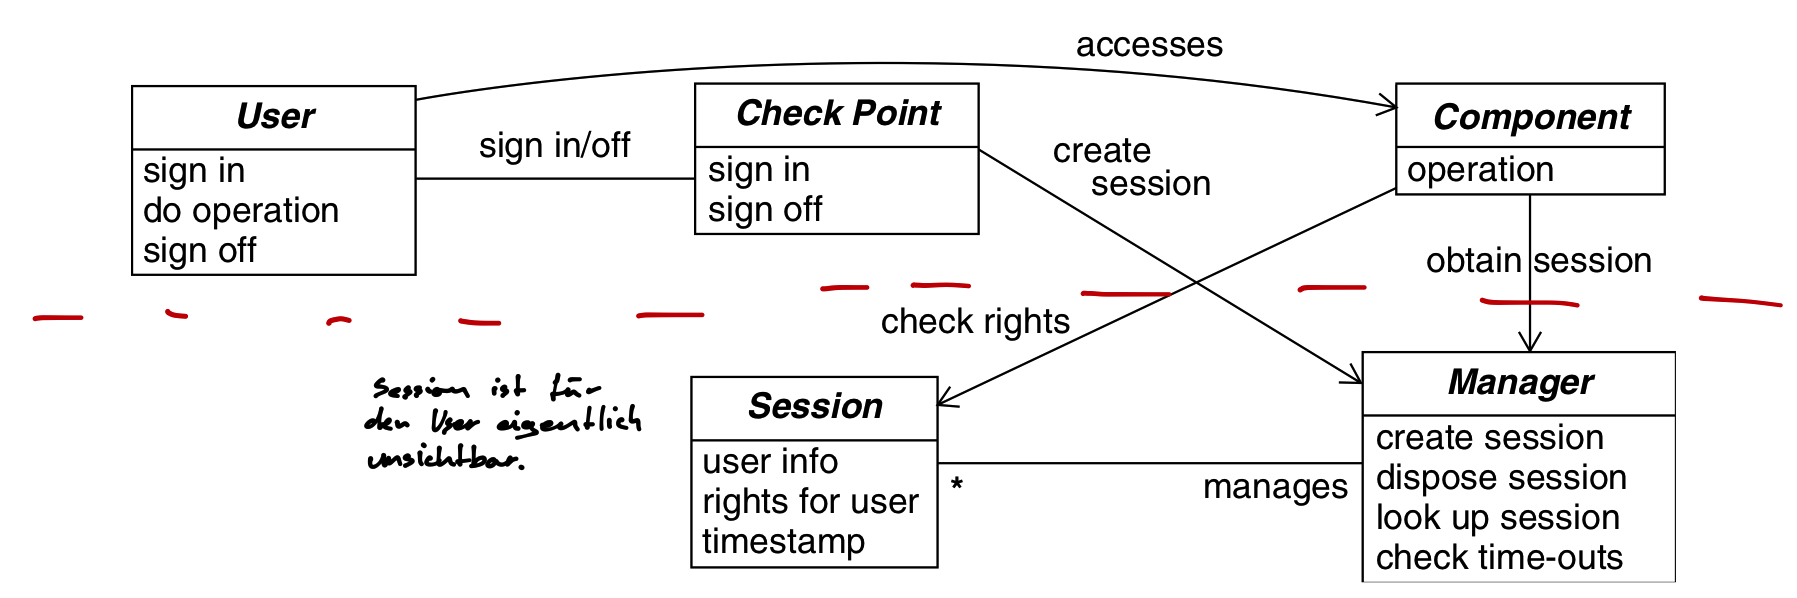
\includegraphics[width=\textwidth]{content/system-access-control-architecture/images/security-session-structure.png}
	\caption{Security Session: Schematischer Aufbau \cite{SecPatterns06}}
\end{figure}

Damit ein Subjekte wiederkehrend mit seinem Session Objekt in Verbindung gebracht werden kann, wird eine Session ID nach aussen publiziert. Dabei ist zu beachten, dass diese für Aussenstehende keine Rückschlüsse auf tatsächliche Inhalte des Session Objektes zulassen.

Das Sequenzdiagramm in Abbildung \ref{fig:securitysessioninteraction} zeigt ein Session Objekt von seiner Erstellung bis hin zu der Zerstörung sobald das Subjekt das System verlässt.

\begin{figure}
	\centering
	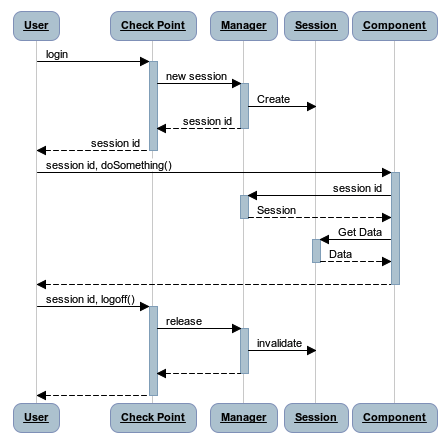
\includegraphics[width=12cm]{content/system-access-control-architecture/images/security-session-interaction.png}
	\caption{Security Session: Interaktion der verschiedenen Akteure}
	\label{fig:securitysessioninteraction}
\end{figure}

\subsubsection*{Implementierung}
\begin{enumerate}
	\item Session Objekt einführen (klar definierte Schnittstelle zur Speicherung von Informationen (Key/Value Pairs, ...))
	\item Einführung eines Session Managers zur Verwaltung der Session Objekte (Zugriff auf Session Objekte mittels Session ID's usw.)
	\item Session Timeouts und die nötig werdenden Aktionen (erneut Anmelden usw.) definieren
	\item Dem Subjekt ermöglichen, sich an einer Session an- und abzumelden (you don't say ;) )
\end{enumerate}

\subsection*{Vorteile}
\begin{itemize}
	\item Klar definierter und zentraler Standort für jegliche Informationen zu einem Subjekt welches sich im System befindet
	\item Komponenten können sich auf ihre Kernfunktionalitäten konzentrieren
\end{itemize}

\subsection*{Nachteile}
\begin{itemize}
	\item Die Verfügbarkeit eines zentralen, globalen Objektes ermuntert möglicherweise zu unschönen Programmiertechniken
	\item Eine Überladung des Session Objektes mit grossen Datenmengen führt zu schlechter Systemperformance
	\item Schlecht gewählte Session ID's lassen möglicherweise Rückschlüsse auf den tatsächlichen Inhalt des Session Objekts
\end{itemize}

\subsection*{Reallife Beispiele}
\begin{itemize}
	\item Jegliche Webapplikationen welche ein Benutzerautentifizierung benötigen greifen auf die Security Session zurück, um einen Stateful-Kontext über das eigentliche zustandslose Medium HTTP zu erzeugen.
	\item Beispiel aus Bachelorarbeit \emph{Alexandre Joly, Michael Weibel \& Manuel Alabor}:\\
	Wird eine Webapplikation auf mehreren CPU-Kernen ausgeführt, kommt es durch Verwendung eines In-Memory-Storages für die Session-Objekte ggf. zu Problemen, da beim Neustart eines Kerns resp. beim Neustart der gesamten Applikation die Sessions verloren gehen. Abhilfe schafft die Auslagerung der Session Objekte wie persistente Datenbanken.
\end{itemize}


\subsection*{Mögliche Prüfungsfragen}
\begin{itemize}
	\item \emph{Wann wird eine Security Session erzeugt?}\\
	Nach erfolgreicher Authentifizierung eines Subjektes. Dies kann bspw. vom Check Point initiiert werden. Optimalerweise würde dieser die Session jedoch nicht selber erzeugen, sondern den Session Manager damit betrauen.
\end{itemize}